\chapter{Model Setup \& Identifiability Conditions}
\label{cha:model-specification}

Given the notation of our thesis in section~\ref{sec:model-setup}, we begin with basic background of the Poisson-Multinomial Equivalence in section~\ref{sec:PME} and EM (Expectation-Maximization) algorithm in section~\ref{sec: em-algorithm-relatives}, which are the core tricks of our algorithms in Chapter~\ref{cha:methodology} and Chapter~\ref{cha:computational-acceleration}. Our model structure is provided in section~\ref{sec:two-level-hierarchy}. In section~\ref{sec:identifiability}, we give the identifiable condition for loading matrix so that the it can be recovered uniquely.

\section{Model Setup}
\label{sec:model-setup}
Our theoretical data structure is hesitated from the yogurt data in~\citet{lee2017poissontrickextensionsfitting}.
Let $\bm{y}_{ij} = (y_{ij1}, \dots, y_{ijQ})^\top \in \mathbb{Z}_{\geq 0}^Q$ denote the count vector representing category-specific choices for observation $i$ in group $j(i)$, spanning $Q$ distinct categories. For each observation $i$, let $j(i) \in \{1, 2, \ldots, J\}$ maps the individual to its corresponding cluster group. We define the group-specific index set as $\mathcal{I}_j = \{i : j(i) = j\}$ with its cardinality denoted by $I_j = |\mathcal{I}_j|$ such that the aggregate sample size satisfies $I = \sum_{j=1}^J I_j$. Here $y_{ij\cdot}$ denotes the Multinomial sum for observation $i$ in group $j(i)$ across $Q$ categories. Each observation carries a covariate vector $\bm{v}_{ij}\in \mathbb{R}^{P}$. We do not include a constant term in $\bm{v}_{ij}$ as category-specific intercepts are carried separately by $\bm{\mu}$.

\section{Poisson-Multinomial Equivalence}
\label{sec:PME}
    
The Poisson-Multinomial Equivalence established by \citet{10.2307/2348134}, states that the Multinomial likelihood conditional on $y_{ij\cdot}$ is exactly equivalent to a product of independent Poisson likelihoods sharing a common additive offset,

\begin{equation}
    \xi_{ij} = \log y_{ij\cdot} - \log\sum_{q=1}^Q \exp(\eta_{ijq}),
    \label{eq:xi_baker}
\end{equation}

The joint Multinomial draw $\bm{y}_{ij} \mid \bm{\lambda}_{j} \sim \mathrm{Multinomial}(y_{ij\cdot}, \bm{p}_{ij})$ is equivalent to $y_{ijq} \mid \bm{\lambda}_{j} \sim \mathrm{Poisson}(\exp(\eta_{ijq} + \xi_{ij}))$ independently for $q = 1, \ldots, Q$, conditional on $y_{ij\cdot}$. We give the definition of $\eta_{ijq}$ and $\bm{p}_{ij}$ in section~\ref{sec:two-level-hierarchy}. The offset~\eqref{eq:xi_baker} absorbs the softmax normalizer and decouples the $Q$ Poisson problems, thus we can solve these $Q$ Poisson independently. 

\citet{lee2017poissontrickextensionsfitting} extended the framework of \citet{10.2307/2348134} by re-conceptualizing the aggregate count $y_{ij\cdot}$, conventionally held fixed as the conditioning variable in the Multinomial likelihood, as itself Poisson-distributed given the group effect $\bm{\lambda}_j$. Marginalizing over this now-random aggregate recovers, exactly, the same factorization into independent Poisson elements across categories $q = 1, \dots, Q$. $\xi_{ij}$ correspondingly shifts from a fixed conditioning quantity into a rate parameter of this induced Poisson distribution on $y_{ij\cdot}$.

The present chapter carries this perspective one step further into the E-step. In the standard Laplace E-step, $\bm{\lambda}_j$ is updated via Newton's method~\ref{eq:newton-method} on the full Multinomial log-posterior $\ell(\bm{\lambda}_j)$. The bottleneck is the rank-$I_j$ outer-product term $\sum_{i \in \mathcal{I}_j} y_{ij\cdot} \bm{p}_{ij} \bm{p}_{ij}^\top$ in Hessian, which arises directly from the softmax normalizer and couples all $Q$ categories, forcing an $O(Q^3)$ linear solve per Newton step. Inspired by the insight of~\citet{lee2017poissontrickextensionsfitting} that the normalization mass can be treated as a random variable rather than a fixed constraint, we introduce $\xi_{ij}$ as an explicit auxiliary optimization variable in the E-step objective. When $\xi_{ij}$ is held fixed during the update of $\bm{\lambda}_j$, the log-sum-exp coupling disappears entirely and the likelihood Hessian reduces to a diagonal matrix, enabling a second Woodbury reduction that cuts the per-step cost from $O(Q(I_j + K))$ to $O(QK^2 + K^3)$.

\section{EM Algorithm \& Relatives}
\label{sec: em-algorithm-relatives}

In order to have a good understanding for further discussion, we briefly review the classical EM algorithm in this section. Then we discuss the models that have the similar structure with our model. 

Let $Y$ and $Z$ be random variables taking values in the sample spaces $\mathcal{Y}$ and $\mathcal{Z}$, respectively. Suppose that the pair $(Y,Z)$ has a joint density function $f_{\theta^{*}}$ that belongs to some parameterized family $\{f_{\theta}\mid \theta\in \Omega
\}$, for a non-empty compact convex set $\Omega$. Rather than observing complete data $(Y,Z)$, we observe only component $Y$.Thus, the component $Z$ corresponds to the missing or latent structure in the data. Our goal is to obtain an estimate of the unknown parameter $\theta^{*}$ via maximum likelihood to compute some $\hat{\theta}\in\Omega$ maximizing the function $\theta\mapsto g_{\theta}(y)$, where

\begin{equation}
    g_{\theta}(y)=\int_{\mathcal{Z}}f_{\theta}(y,z)\,dz
    \label{eq:classical-em-integral}
\end{equation}
is the density function of the observed variable $Y$.

In many settings, computing log likelihood $\log f_{\theta}(y,z)$ of both latent variables and observed data is easier and computationally cheaper than evaluating the log likelihood of the observed data itself. The EM algorithm is well-suited to such settings. For each $\theta\in\Omega$, let $k_{\theta}(z\mid y)$ denote the conditional density of $z$ given by $y$, then the log likelihood at $\theta^{'}\in\Omega$ can be lower bounded using Jensen's inequality
\begin{equation}
    \log g_{\theta'}(y) \;\ge\; \underbrace{\int_{\mathcal{Z}} k_\theta(z \mid y) \log f_{\theta'}(y,z)\, dz}_{Q(\theta' \mid \theta)} \;-\; \int_{\mathcal{Z}} k_\theta(z \mid y) \log k_\theta(z \mid y)\, dz,
    \label{eq:classical-em-jensen}
\end{equation}
the equality holds when $\theta=\theta^{'}$. Thus, we have a family of lower bounds on the log likelihood, denoted by $Q(\cdot\mid \cdot)$. We maximize this lower bound in M-step
\begin{equation}
    \theta^{(t+1)}=\arg\max_{\theta^{'}\in\Omega}Q(\theta^{'}\mid \theta^{(t)}),
    \label{eq:em-m-step}
\end{equation}
and then reevaluates the lower bound at the new parameter value in E-step.

\section{Two-Level Hierarchy}
\label{sec:two-level-hierarchy}

\begin{figure}[H]
    \centering
    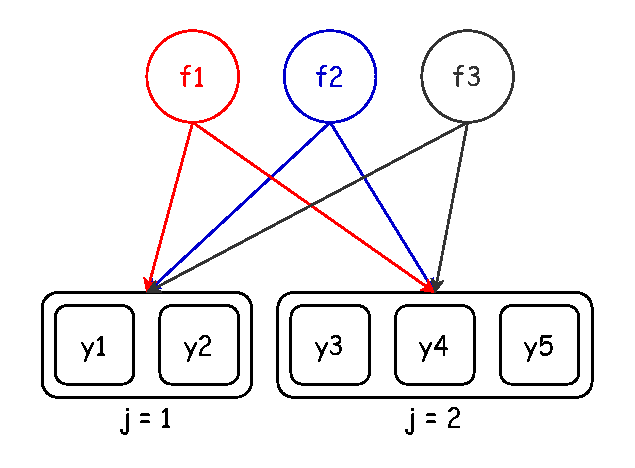
\includegraphics[width=0.48\textwidth]{figs/data_structure.drawio.pdf}
    \caption{Data Structure: Orthogonal case that each latent factors $f1$–$f3$ is independent to others. Each directed edge represents that a latent factor affects the response variable $\bm{y}_{ij}$ for $j\in\{1,2\}$. Notice that each latent factor affects all groups publicly.}
    \label{fig:data_structure}
\end{figure}

\paragraph*{Observation Level}
Conditional on the total count $y_{ij\cdot}=\sum_{q=1}^{Q}y_{ijq}$ and group-level random effect $\bm{\lambda}_{j}\in \mathbb{R}^{Q}$, each observation follows a Multinomial distribution:
\begin{equation}
    \bm{y}_{ij} \mid  y_{ij\cdot} , \bm{\lambda}_{j}
    \sim \operatorname{Multinomial}\left(y_{ij\cdot},\, \bm{p}_{ij}\right), \quad p_{ijq}=\frac{\exp(\eta_{ijq})}{\sum_{q'=1}^{Q}\exp(\eta_{ijq'})},
    \label{eq:conditional-pm}
\end{equation}
where the log-linear predictor is:
\begin{equation}
    \eta_{ijq}=\mu_{q}+\bm{v}_{ij}^{\top}\bm{\phi}_{q}+
    \lambda_{jq}, \quad q=1,2,\dots, Q,
    \label{eq:linear-predictor}
\end{equation}
and $\mu_{q}\in\mathbb{R}$ is the category-specific intercept, $\bm{\phi}_{q}\in\mathbb{R}^{P}$ is the vector of covariate effects for category $q$, and $\lambda_{jq}$ is the contribution of group $j$ to the log-relative-rate of category $q$. Equation~\eqref{eq:linear-predictor} extends the linear predictor of DMR \citep{Taddy_2015} and of the grouped Poisson-trick extension of \citet{lee2017poissontrickextensionsfitting}; the three models differ only in the distribution placed on $\bm{\lambda}_{j}$.

The softmax link in \eqref{eq:conditional-pm} is invariant under the shift $\eta_{ijq}\mapsto\eta_{ijq}+c_{ij}$ for any constant $c_{ij}$ common to all categories, so the intercepts $\bm{\mu}=(\mu_{1},\dots,\mu_{Q})$ are identified only up to an additive constant. We remove this indeterminacy by imposing the reference constraint $\mu_{1}=0$ (equivalently, a sum-to-zero constraint $\sum_{q}\mu_{q}=0$); identification is in any case restored automatically by the Poisson representation introduced below, in which each category carries its own offset.

Throughout, the total count $y_{ij\cdot}$ is treated as ancillary for $(\bm{\mu},\bm{\Phi},\bm{\lambda}_{j})$: its generating mechanism is assumed to carry no information about these parameters beyond what is already encoded in them, so that conditioning on $y_{ij\cdot}$ in \eqref{eq:conditional-pm} loses no relevant information. This is the standard convention in Multinomial regression, but it is not automatic, and we do not pursue a joint volume--composition model here. We stress that ancillarity is a statement about information, not about determinism: the total remains a random quantity, but its distribution carries no additional information about $(\bm{\mu},\bm{\Phi},\bm{\lambda}_{j})$. In Section~\ref{sec:PME} we exploit the Poisson-Multinomial equivalence to represent each $y_{ijq}$ as an independent Poisson variate whose offset $\xi_{ij}$ absorbs the (random) total; the Multinomial conditional in \eqref{eq:conditional-pm} is recovered exactly upon conditioning on $y_{ij\cdot}$. The two views are therefore consistent, and $\xi_{ij}$ is a computational device rather than a modelling assumption about the total.

\paragraph*{Group Level}

The group random effects are assumed independently and identically distributed:

\begin{equation}
    \bm{\lambda}_{j}\sim \mathcal{N}(\bm{0},\bm{\Sigma}), \quad \bm{\Sigma}=\mathbf{BB}^{\top}+\mathbf{D},
    \label{eq: Overall notation structure}
\end{equation}
where $\mathbf{B}\in \mathbb{R}^{Q\times K}$ is the factor loadings matrix and $\mathbf{D}$ is the variance. Equivalently, in the factor regression form:

\begin{equation}
    \bm{\lambda}_{j}=\mathbf{B}\mathbf{f}_{j}+\bm{\epsilon}_{j}, \quad \mathbf{f}_{j}\sim \mathcal{N}(\bm{0},\bm{I}_{K}), \quad \bm{\epsilon}_{j}\sim \mathcal{N}(\bm{0},\mathbf{D}),
    \label{eq: Detailed notation structure}
\end{equation}
so that $\lambda_{jq}=\mathbf{b}_{q}^{\top}\mathbf{f}_{j}+\epsilon_{jq}$, where $\mathbf{b}_{q}$ is the q-th row of $\mathbf{B}$. We use \ref{eq: Overall notation structure} for inference and \ref{eq: Detailed notation structure} for interpretation.

For the error matrix $\mathbf{D}$, we do the analysis with the assumption $\mathbf{D}=\sigma^{2}\mathbf{I}_{Q}$ with $\sigma^{2} >0$ instead of taking the diagonal assumption $\mathbf{D}=\text{diag}(d_{1}^{2},\dots,d_{Q}^{2})$ with entries $d_{q}>0$. The chosen form of the error is selected to simplify the computation when we introduce the Woodbury equality in Chapter~\ref{cha:}, whose result is more complex to explain in diagonal assumption.

\begin{remark}[Variance decomposition]
The variance of the log-relative-rate of category $q$ decomposes as 
\begin{equation*}
    \operatorname{Var}(\lambda_{jq})=\|\mathbf{b}_{q}\|^{2}+\sigma^{2},
\end{equation*}
where $\|\mathbf{b}_{q}\|^{2}$ captures the structured factor component and $\sigma^2$ the idiosyncratic component. The ratio $\|\mathbf{b}_{q}\|^2/(\|\mathbf{b}_{q}\|^2+\sigma^2)$ quantifies the proportion of between-group variation in category $q$ explained by the latent factors. 
\end{remark}

\section{Identifiability}
\label{sec:identifiability}

In many settings, we categorize the latent factors into orthogonal and non-orthogonal\citet{@articleCui_2026}. Orthogonal factors are assumed to be independent, which illustrates the relationship of factors in our group random effects \ref{eq: Detailed notation structure}. In this section, we present the conditions that guarantee the rotational identifiability, which are treated as given in the rest of the thesis. 

Both linear latent factor model and the generalized latent factor model suffer form rotational indeterminacy, which is the primary source of non-identification in factor analysis (\citet{BAI2012}, \citet{BAI201318}). The factor structure \ref{eq: Detailed notation structure} is subject to classical indeterminacy, which includes both rotational and sign indeterminacy. For any $K\times K$ orthogonal matrix $\mathbf{V}$, the substitution $(\mathbf{B},\mathbf{f}_{j})\to (\mathbf{BV},\mathbf{V}^{\top}\mathbf{f}_{j})$ leaves the distribution of $\bm{\lambda}_{j}$ unchanged. Also, the substitution $(\mathbf{b}_{k},\mathbf{f}_{j})\to (-\mathbf{b}_{k},-\mathbf{f}_{j})$ product of $\mathbf{b}_{q}\mathbf{f}_{k}$ is the same as $(-\mathbf{b}_{q})(-\mathbf{f}_{k})$. 

A more common approach in applications to ensure identifiability is to prescribe zeros in the loading matrix $\mathbf{B}$. Under our orthogonal assumption, the additional $K(K-1)/2$ constrains are imposed by fixing $K(K-1)/2$ entries to be zeros. Interestingly, the Example~\ref{eg:no-rotational} shows that not all configurations of the $K(K-1)/2$ zeros ensure identifiability.

\begin{example}
    This example was given by~\citet{Cui2026}. We set $K=3$ and assign at least 3 zeros in loading matrix $\mathbf{B}$. Consider the loading matrix $\mathbf{B}$ and the orthogonal transformation matrix $\mathbf{G}$,
    \begin{equation*}
        \mathbf{B}_{[1:2,]}=
        \begin{pmatrix}
            0 & a_{12} & a_{13} \\
            a_{21} & 0 & 0 
        \end{pmatrix}, \quad \mathbf{G}_{\theta}=
        \begin{pmatrix}
            1 & 0 & 0 \\
            0 & \cos \theta & \sin \theta \\
            0 & -\sin \theta & \cos \theta
        \end{pmatrix}.
    \end{equation*}
    For any $\theta$, 
    \begin{equation*}
        [\mathbf{B}\mathbf{G}_{\theta}]_{[1:2,]}
        =
        \begin{pmatrix}
            0 & *_{12} & *_{13} \\
            a_{21} & 0 & 0 
        \end{pmatrix}.
    \end{equation*}
    
    For any $\theta$, the zero pattern of $[\mathbf{B}\mathbf{G}_{\theta}]_{[1:2,]}$ retains the same as $\mathbf{B}_{[1:2,]}$. Thus, the above transformation matrix $\mathbf{G}_{\theta}$ leaves the factor covariance matrix unchanged, which is not rotationally identifiable under this constraint. 
    \label{eg:no-rotational}
\end{example}

Example~\ref{eg:no-rotational} shows that a necessary condition for identifiability is that no two columns of the loading matrix share the same zero pattern. To avoid these cases, we consider the following sufficient condition that covers many commonly used identifiability constraints. Thus, we give the positive lower triangular constraint to recover the true value of matrix $\mathbf{B}$, 

\begin{equation}
    b_{qk}=0 \text{ for } q<k,
    \label{eq: PLT1}
\end{equation}
\begin{equation}
    b_{kk}>0 \text{ for }k=1,2,\dots ,K,
    \label{eq:PLT2}
\end{equation}
which solves the rotationally indeterminacy by condition~\ref{eq: PLT1} and sign indeterminacy by condition~\ref{eq:PLT2}. \citet{Cui2026} had proved many sufficient constraints, and we adapt their IC$^{(2)}$ with orthogonal latent factors in factor analysis.

